\red{Здесь схема оптики для подготовки лучей твизеров, схема подключения и генерации}.



\begin{figure}
    \centering
    \addletter{195}{a} \phantom{4}
    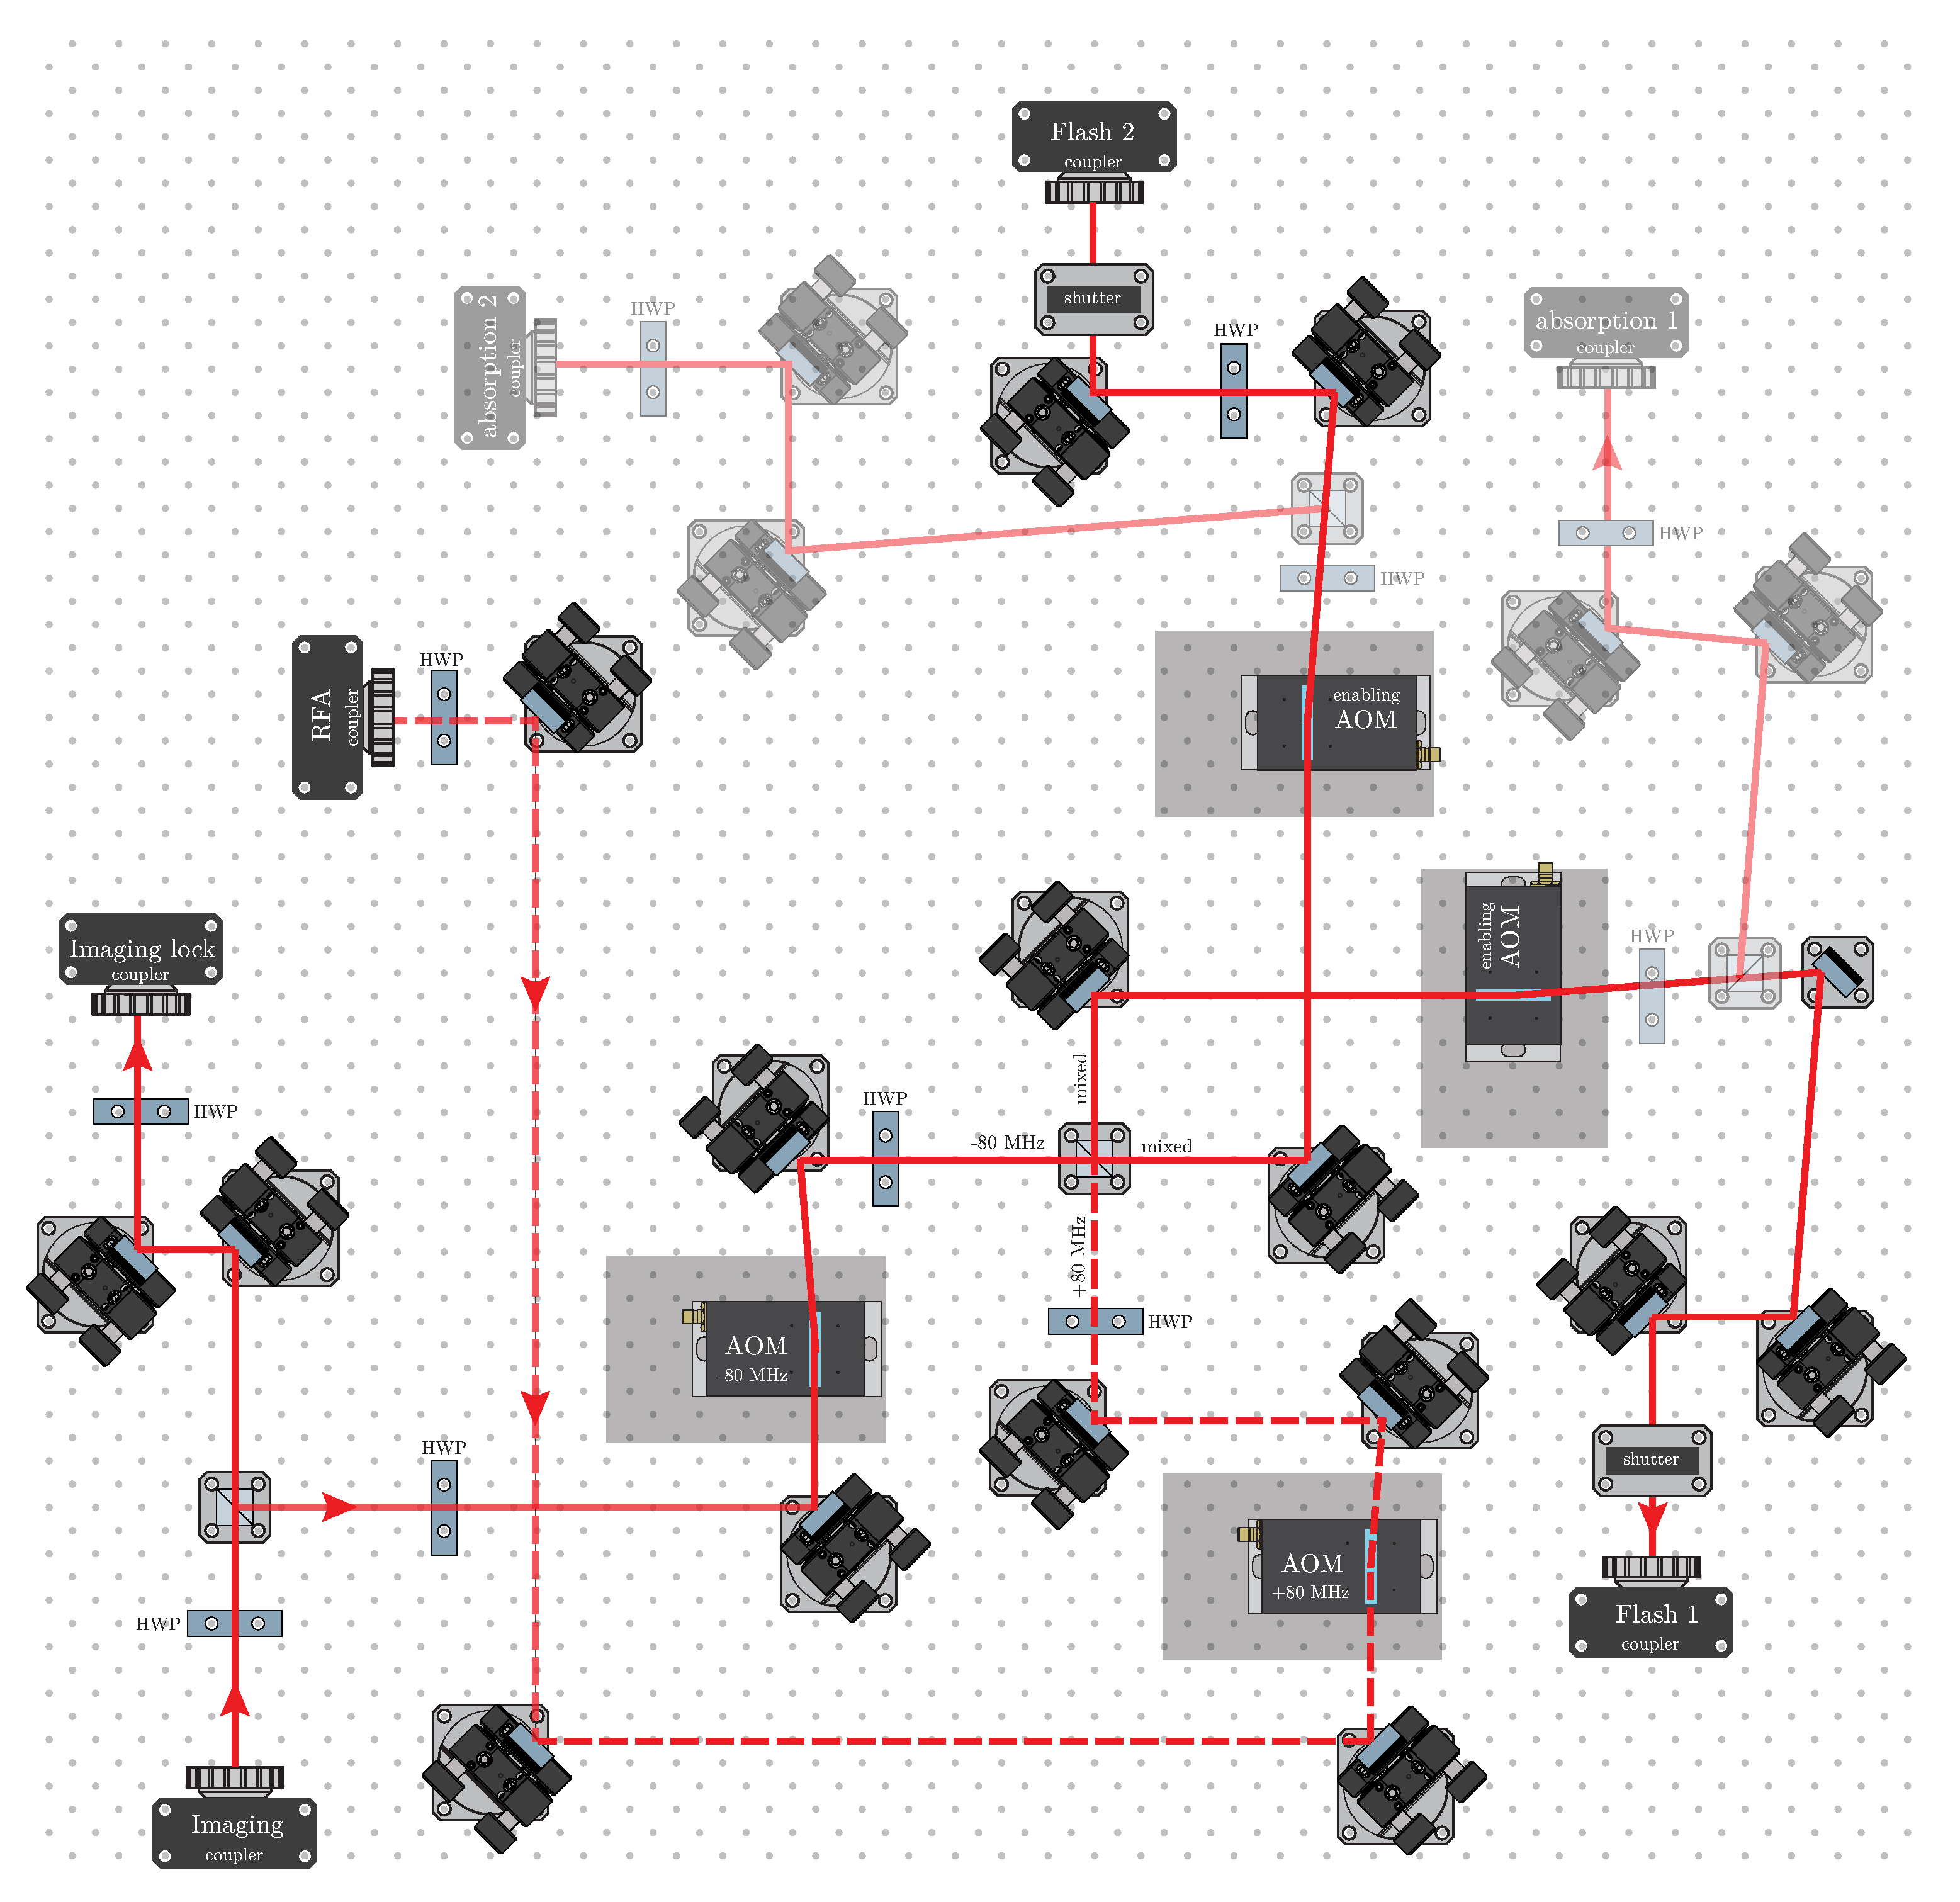
\includegraphics[width=0.4\textwidth]{fig-ai/flashing-distribution-scheme.pdf}
    \hspace{10 mm} 
    \addletter{195}{b} \phantom{4}
    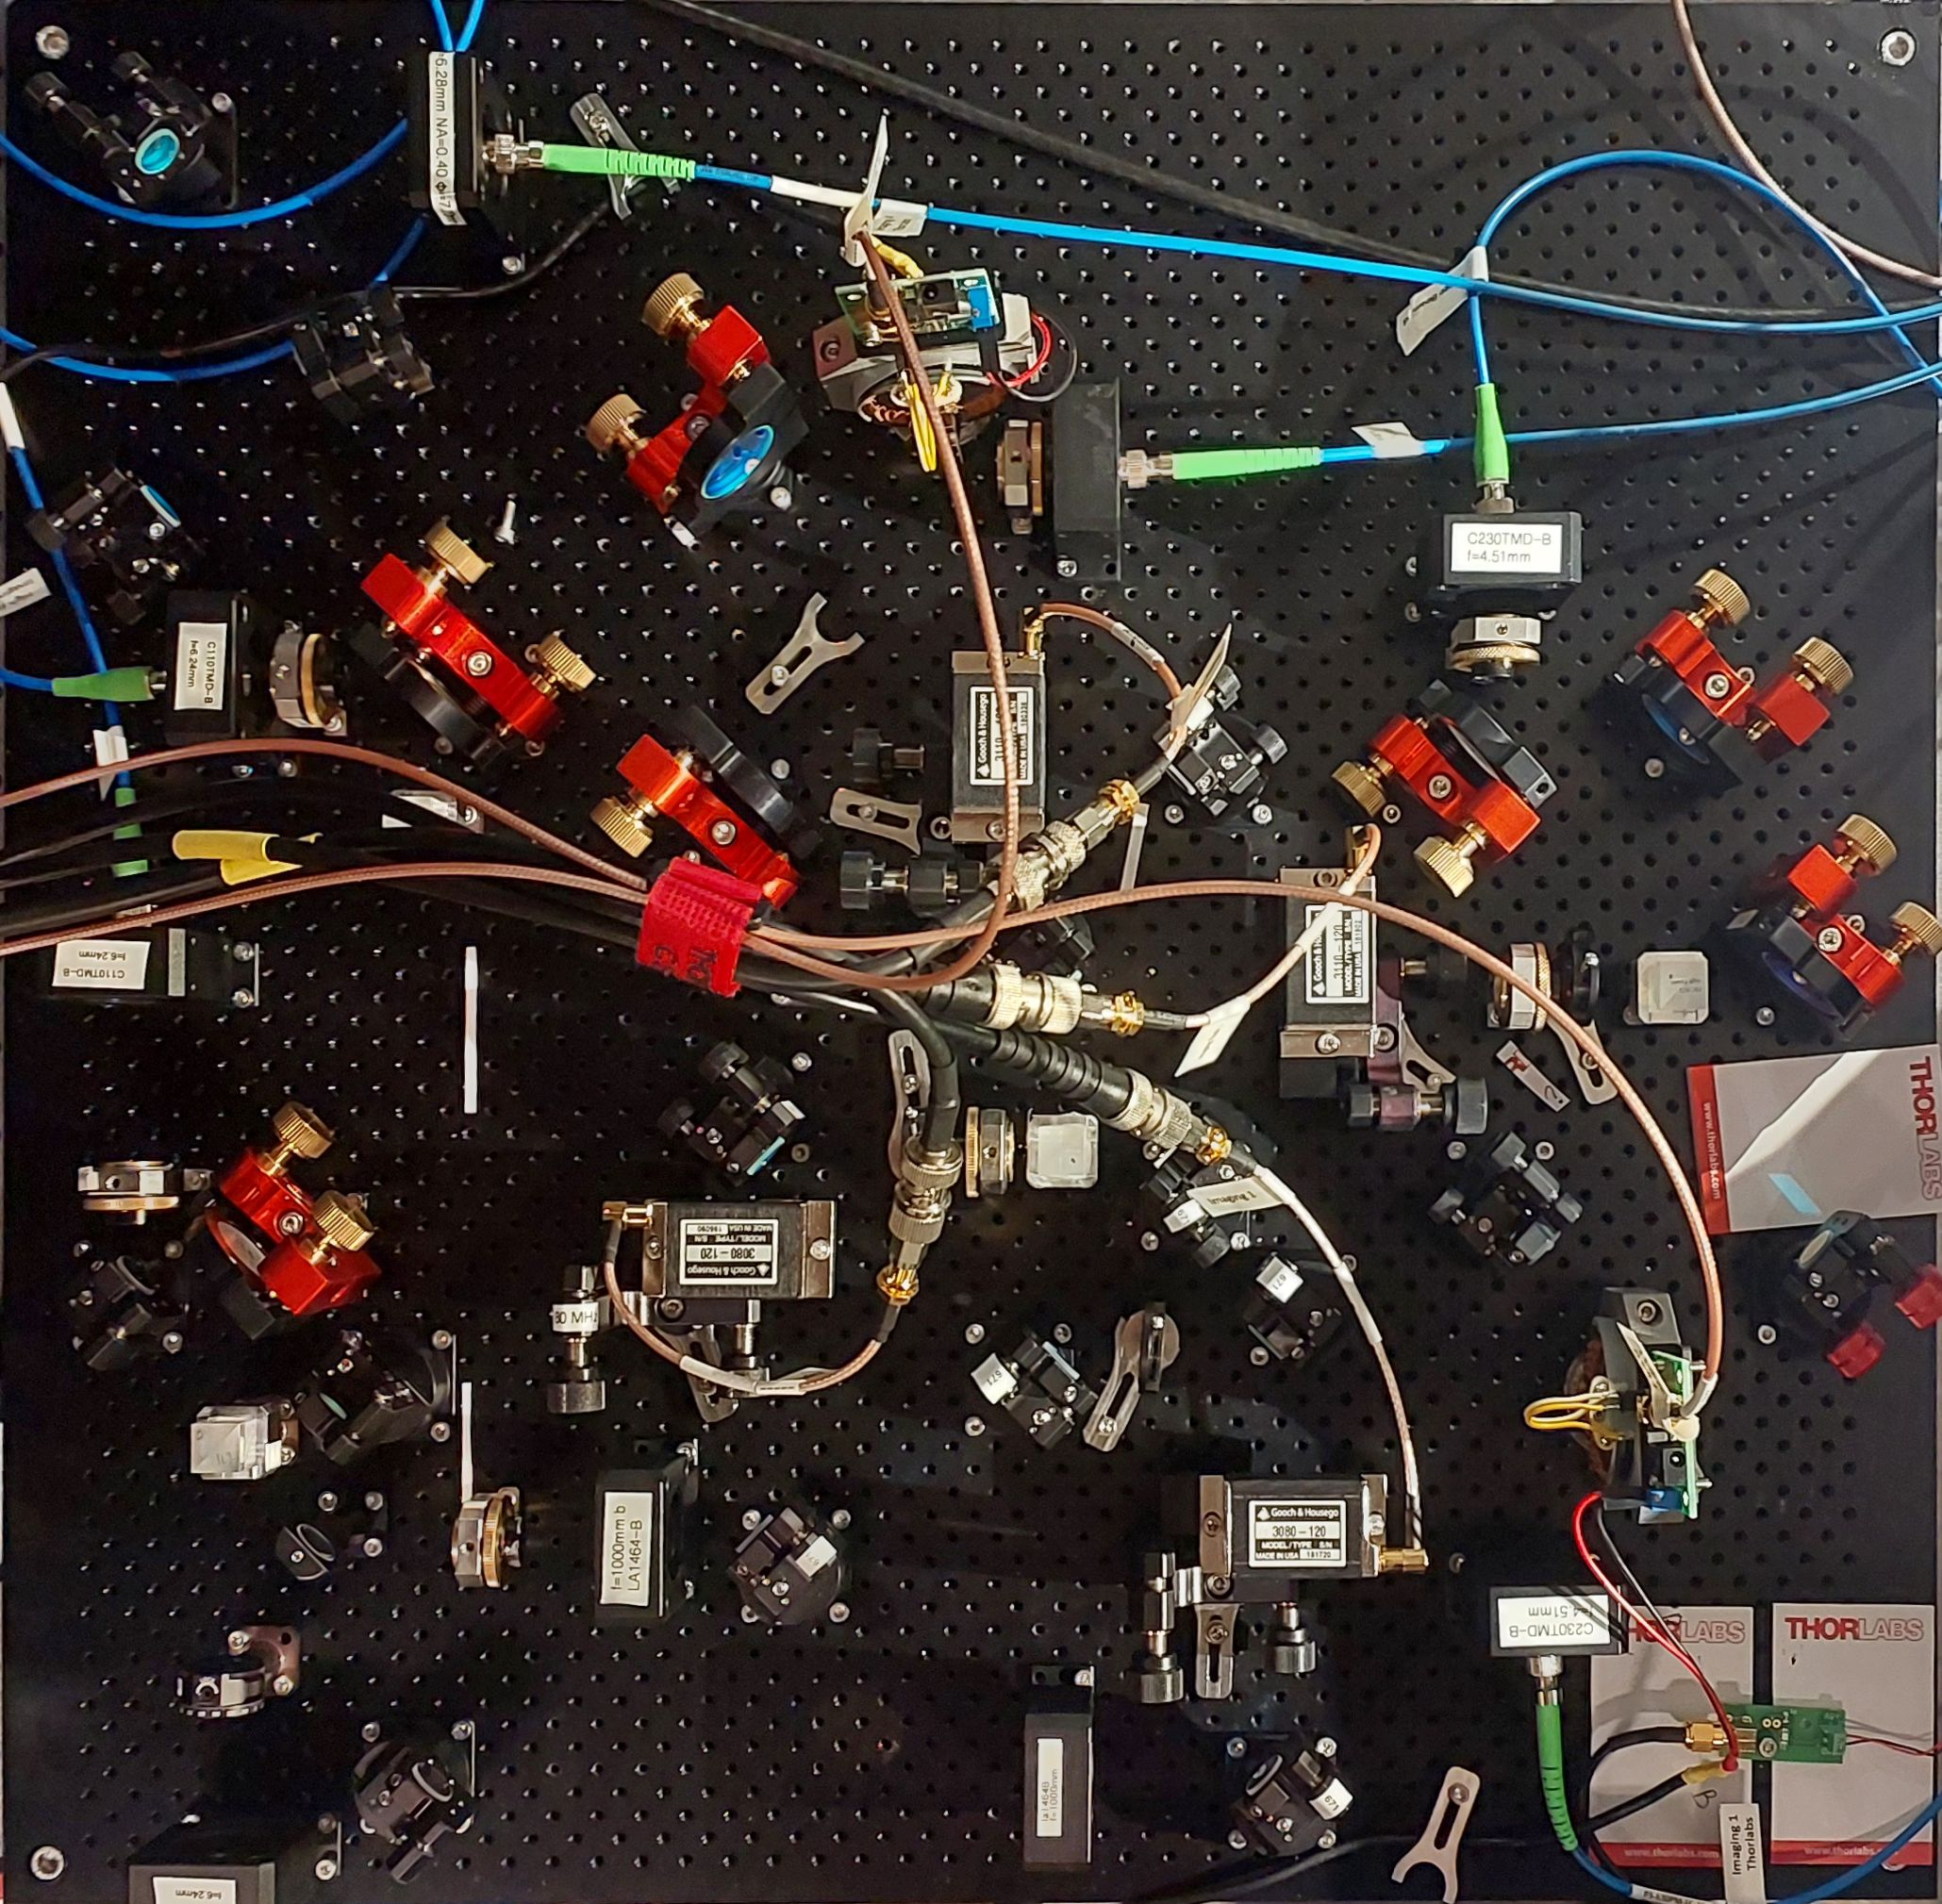
\includegraphics[width=0.4\textwidth]{imgs/flashing-distribution-img.jpg}

    \addletter{90}{c}
    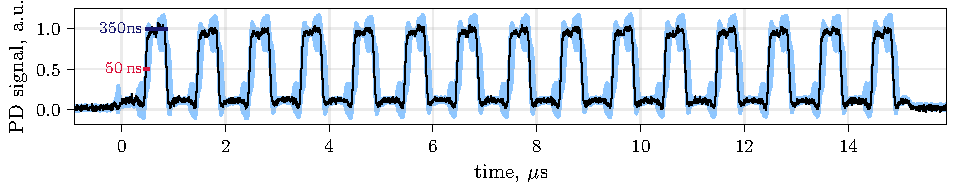
\includegraphics{fig-py/flashing-oscilloscope.pdf}

    \caption{
        \textbf{Distribution board for flashing}. 
        a) Optical layout of the board used to combine and control light for free-space imaging states $\ket{3}$ and $\ket{6}$.
        b) Experimental implementation.
        c) PD signal of the flashing measured on an oscilloscope (black -- a single experimental run, blue -- the standard deviation over 20 runs, red -- rise time).
    }
    \label{fig:flashing}
\end{figure}

